\documentclass[tikz,border=2pt]{standalone}
\usepackage{amsmath,amssymb}
\usepackage{tikz}
\usetikzlibrary{arrows.meta}

\begin{document}
% The complex plane with Cartesian coordinates: z = x + yi sits at the point (x, y).
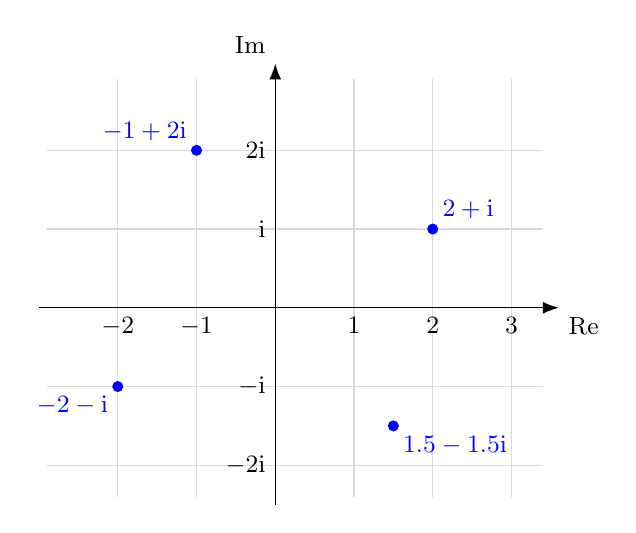
\begin{tikzpicture}[every node/.style={font=\small}, >={Latex[length=2mm]}]
	\draw[gray!30, step=1] (-2.9,-2.4) grid (3.4,2.9);
	\draw[->] (-3,0) -- (3.6,0) node[below right] {$\mathrm{Re}$};
	\draw[->] (0,-2.5) -- (0,3.1) node[above left] {$\mathrm{Im}$};
	\foreach \x in {-2,-1,1,2,3} {\node[below, font=\small] at (\x,0) {$\x$};}
	\foreach \y/\l in {-2/{-2\mathrm{i}},-1/{-\mathrm{i}},1/{\mathrm{i}},2/{2\mathrm{i}}} {\node[left, font=\small] at (0,\y) {$\l$};}
	\fill[blue] (2,1) circle (2pt) node[above right] {$2+\mathrm{i}$};
	\fill[blue] (-1,2) circle (2pt) node[above left] {$-1+2\mathrm{i}$};
	\fill[blue] (-2,-1) circle (2pt) node[below left] {$-2-\mathrm{i}$};
	\fill[blue] (1.5,-1.5) circle (2pt) node[below right] {$1.5-1.5\mathrm{i}$};
\end{tikzpicture}
\end{document}
